\chapter{Analisi dei requisiti}
\label{cap:analisi-requisiti}

\intro{In questo capitolo viene esposta l'analisi dei requisiti effettuata durante lo stage, dove si
 vanno ad illustrare le funzionalità tramite casi d'uso e requisiti identificati, con l'obiettivo di creare un'immagine
 più chiara e definita del sistema.
 }\\

\section{Descrizione dell'applicazione}

\section{Casi d'uso}

Per lo studio dei casi di utilizzo del prodotto sono stati creati dei diagrammi.
I diagrammi dei casi d'uso (in inglese \emph{Use Case Diagram}) sono diagrammi di tipo \gls{uml} dedicati alla descrizione delle funzioni o servizi offerti da un sistema, così come sono percepiti e utilizzati dagli attori che interagiscono col sistema stesso.
Essendo il progetto finalizzato alla creazione di un tool per l'automazione di un processo, le interazioni da parte dell'utilizzatore devono essere ovviamente ridotte allo stretto necessario. Per questo motivo i diagrammi d'uso risultano semplici e in numero ridotto.

% \begin{figure}[!h] 
%     \centering 
%     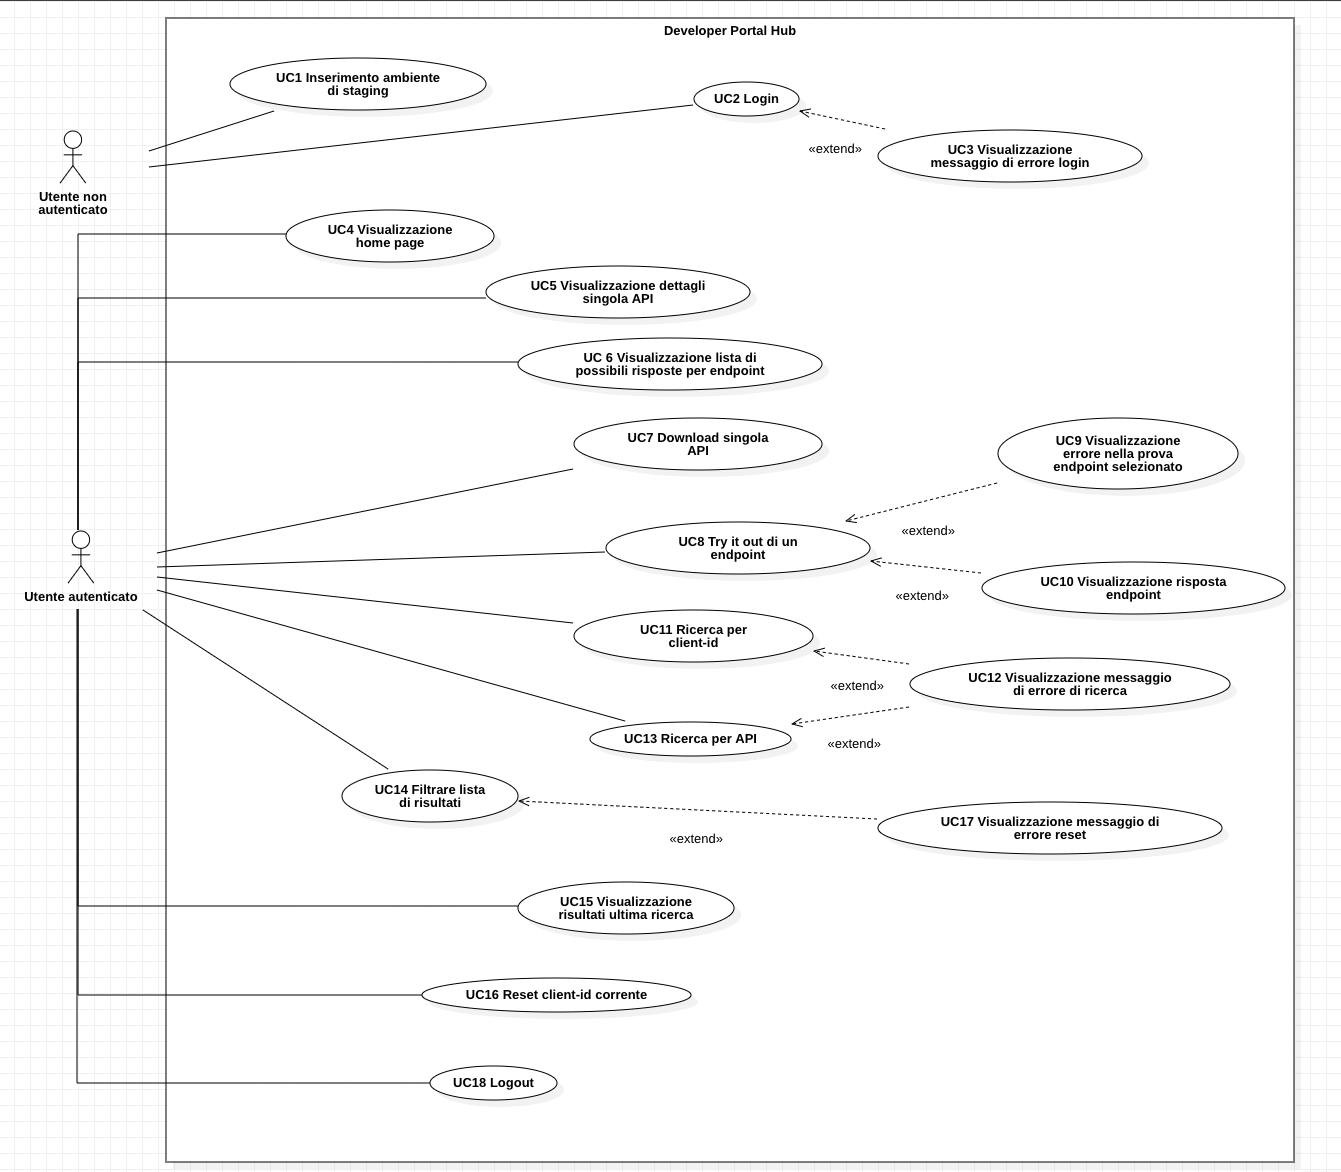
\includegraphics[width=0.9\columnwidth]{usecase/scenario-principale} 
%     \caption{Use Case - UC0: Scenario principale}
% \end{figure}

\begin{usecase}{1}{Login}\label{uc:login}
\usecaseactors{Utente non autenticato}
\usecasepre{}
\begin{itemize}
    \item L'utente possiede un account valido per autenticazione tramite microsoft 365;
    \item L'utente è all'interno del gruppo autorizzato per il login al portale.
\end{itemize}
\usecasedesc{L'utente vuole accedere al portale e deve inserire le proprie credenziali per accedervi}
\usecasepost{L'utente è autenticato correttamente e può procedere con l'utilizzo di tutte le funzionalità disponibili all'interno del portale}
\usecasemain{}
\begin{itemize}
    \item L'utente inserisce le proprie credenziali di accesso.
\end{itemize}


\end{usecase}

\section{Tracciamento dei requisiti}

Da un'attenta analisi dei requisiti e degli use case effettuata sul progetto è stata stilata la tabella che traccia i requisiti in rapporto agli use case.\\
% Sono stati individuati diversi tipi di requisiti e si è quindi fatto utilizzo di un codice identificativo per distinguerli.\\
% Il codice dei requisiti è così strutturato R(F/Q/V)(N/D/O) dove:
% \begin{enumerate}
% 	\item[R =] requisito
%     \item[F =] funzionale
%     \item[Q =] qualitativo
%     \item[V =] di vincolo
%     \item[N =] obbligatorio (necessario)
%     \item[D =] desiderabile
%     \item[Z =] opzionale
% \end{enumerate}
% Nelle tabelle \ref{tab:requisiti-funzionali}, \ref{tab:requisiti-qualitativi} e \ref{tab:requisiti-vincolo} sono riassunti i requisiti e il loro tracciamento con gli use case delineati in fase di analisi.

% \newpage

% \begin{table}%
% \caption{Tabella del tracciamento dei requisti funzionali}
% \label{tab:requisiti-funzionali}
% \begin{tabularx}{\textwidth}{lXl}
% \hline\hline
% \textbf{Requisito} & \textbf{Descrizione} & \textbf{Use Case}\\
% \hline
% RFN-1     & L'interfaccia permette di configurare il tipo di sonde del test & UC1 \\
% \hline
% \end{tabularx}
% \end{table}%

% \begin{table}%
% \caption{Tabella del tracciamento dei requisiti qualitativi}
% \label{tab:requisiti-qualitativi}
% \begin{tabularx}{\textwidth}{lXl}
% \hline\hline
% \textbf{Requisito} & \textbf{Descrizione} & \textbf{Use Case}\\
% \hline
% RQD-1    & Le prestazioni del simulatore hardware deve garantire la giusta esecuzione dei test e non la generazione di falsi negativi & - \\
% \hline
% \end{tabularx}
% \end{table}%

% \begin{table}%
% \caption{Tabella del tracciamento dei requisiti di vincolo}
% \label{tab:requisiti-vincolo}
% \begin{tabularx}{\textwidth}{lXl}
% \hline\hline
% \textbf{Requisito} & \textbf{Descrizione} & \textbf{Use Case}\\
% \hline
% RVO-1    & La libreria per l'esecuzione dei test automatici deve essere riutilizzabile & - \\
% \hline
% \end{tabularx}
% \end{table}%
